\documentclass{beamer}
\usepackage[utf8]{inputenc}
\usepackage{amsmath, pdfpages, pdflscape, lscape, color, listings, hyperref, amssymb, graphicx,textcomp,varioref, afterpage, subcaption, float, bm, tikz, multicol} 

\global
\newcommand{\Fig}[1]{Figure \ref{#1}}
\newcommand{\fig}[1]{figure \ref{#1}}
\newcommand{\tab}[1]{table \ref{#1}}
\newcommand{\eq}[1]{equation \ref{#1}}
\newcommand{\Eq}[1]{Equation \ref{#1}}
\newcommand{\alg}[1]{algorithm \ref{#1}}
\newcommand{\Alg}[1]{Algorithm \ref{#1}}
\newcommand{\chp}[1]{chapter  \ref{#1}}
\newcommand{\Chp}[1]{Chapter  \ref{#1}}
\newcommand{\e}[1]{\cdot 10^{#1}}
\newcommand{\h}{\hbar}
\newcommand{\der}[2]{\frac{\partial #1}{\partial #2}}
\newcommand{\dder}[2]{\frac{\partial^2 #1}{\partial #2^2}}
\newcommand{\p}{\boldsymbol{P}}
\newcommand{\q}{\boldsymbol{q}}
\newcommand{\norm}[1]{\left\lVert#1\right\rVert}
\newcommand{\coef}[2]{\frac{\langle #1,#2\rangle_Q}{\norm{#2}^}}


\newenvironment{test}[1]
{
 \usebackgroundtemplate{}
 \color{gray!30!black}
   \begin{tikzpicture}[remember picture, overlay]
     \node[anchor = center, opacity=.25] (image) at (current page.center) {
\includegraphics[scale=0.25]{chaospy_logo.jpg}};
   \end{tikzpicture}
 \begin{frame}[fragile,enviroment=chaospy]
   
}
{
 \end{frame}
}

\lstset{
escapeinside=||
}


\newenvironment{chaospy}[1]
{\color{gray!30!black}
     \color{gray!30!black}
     \usebackgroundtemplate{
   \begin{tikzpicture}[remember picture, overlay]
     \node[anchor = center, opacity=.25] (image) at (current page.center) {
\includegraphics[scale=0.25]{chaospy_logo.jpg}};
   \end{tikzpicture}}
     \begin{frame}[fragile,environment=chaospy]
    \frametitle{{#1}}}
{\end{frame}}


\definecolor{keywords}{RGB}{255,0,90}
\definecolor{comments}{RGB}{0,0,113}
\definecolor{red}{RGB}{160,0,0}
\definecolor{green}{RGB}{0,150,0}
 
\usetheme{kalkulo}

\graphicspath{{./figures/}}


\title{Polynomial chaos expansions: Solutions}
\author{Jonathan Feinberg and Simen Tennøe}


\begin{document}


\begin{frame}
  \maketitle
\end{frame}

 \begin{chaospy}{Traveling with constant velocity.}
 \scriptsize
 \begin{lstlisting}[language=Python]
def s(t, v):
    return v*t

v = cp.Normal(5,1)
t = np.linspace(0,10,1000)
M = 5

P = cp.orth_ttr(M, v)
nodes, weights = cp.generate_quadrature(M+1, v, rule="G")
solves = [s(t, n) for n in nodes.T]
U_hat = cp.fit_quadrature(P, nodes, weights, solves)

E = cp.E(U_hat, v)
Var = cp.Var(U_hat, v)
\end{lstlisting}
\end{chaospy}


\begin{frame}
 \frametitle{Traveling with constant velocity.}
  \begin{figure}
  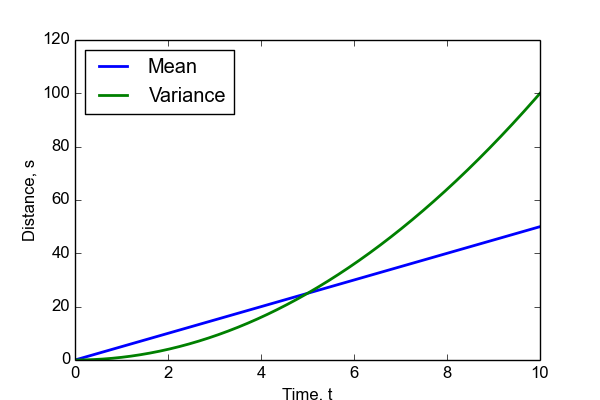
\includegraphics[width=0.85\textwidth]{solution1.png}
 \end{figure}
\end{frame}

 \begin{chaospy}{Traveling with constant acceleration, classical Monte Carlo integration.}
 \scriptsize
 \begin{lstlisting}[language=Python]
def s(t, v0, a):
    return v0*t + 0.5*a*t**2

N = 1000
v0 = cp.Uniform(1,2)
a = cp.Beta(2,2)
t = np.linspace(0,10,1000)

samples_v0 = v0.sample(N)
samples_a = a.sample(N)

distance = np.array([s(t,v0_,a_) for v0_,a_ \
                     in zip(samples_v0.T, samples_a.T)])
E = np.sum(distance,0)/N
Var = np.sum(distance**2,0)/N - E**2
\end{lstlisting}
\end{chaospy}


\begin{frame}
 \frametitle{Traveling with constant acceleration, classical Monte Carlo integration.}
  \begin{figure}
  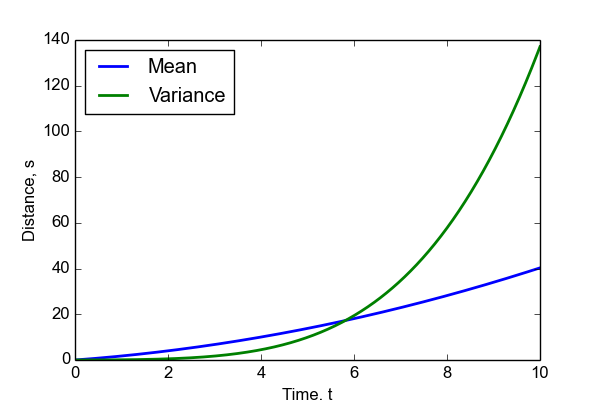
\includegraphics[width=0.85\textwidth]{solution2.png}
 \end{figure}
\end{frame}




 \begin{chaospy}{Traveling with constant acceleration, Quasi-Monte Carlo using \underline{S}obol sequence.}
 \scriptsize
 \begin{lstlisting}[language=Python]
def s(t, v0, a):
    return v0*t + 0.5*a*t**2

N = 1000
v0 = cp.Uniform(1,2)
a = cp.Beta(2,2)
t = np.linspace(0,10,1000)

samples_v0 = v0.sample(N, "S")
samples_a = a.sample(N, "S")

distance = np.array([s(t,v0_,a_) for v0_,a_ \
                     in zip(samples_v0.T, samples_a.T)])
E = np.sum(distance,0)/N
Var = np.sum(distance**2,0)/N - E**2
\end{lstlisting}
\end{chaospy}



\begin{frame}
 \frametitle{Traveling with constant acceleration, Quasi-Monte Carlo using \underline{S}obol sequence.}
  \begin{figure}
  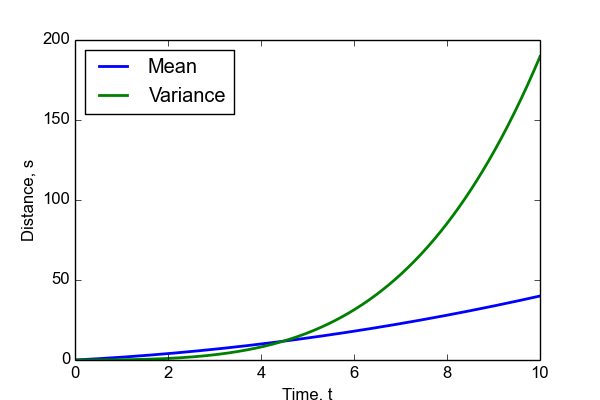
\includegraphics[width=0.85\textwidth]{solution3.png}
 \end{figure}
\end{frame}




 \begin{chaospy}{Traveling with constant acceleration, pseudo-spectral projection with full tensor grid \underline{G}aussian quadrature.}
 \scriptsize
 \begin{lstlisting}[language=Python]
def s(t, v0, a):
    return v0*t + 0.5*a*t**2

v0 = cp.Uniform(1,2)
a = cp.Beta(2,0.5)
dist = cp.J(v0,a)

t = np.linspace(0,10,1000)
M = 5

P = cp.orth_ttr(M, dist)
nodes, weights = cp.generate_quadrature(M+1, dist, rule="G")
solves = [s(t, *n) for n in nodes.T]
U_hat = cp.fit_quadrature(P, nodes, weights, solves)

E = cp.E(U_hat, dist)
Var = cp.Var(U_hat, dist)
\end{lstlisting}
\end{chaospy}



\begin{frame}
 \frametitle{Traveling with constant acceleration, pseudo-spectral projection with full tensor grid \underline{G}aussian quadrature.}
  \begin{figure}
  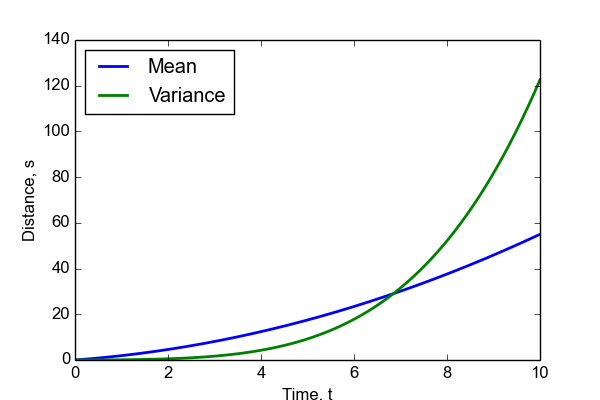
\includegraphics[width=0.85\textwidth]{solution4.png}
 \end{figure}
\end{frame}



 \begin{chaospy}{Traveling with constant acceleration, pseudo-spectral projection with \underline{C}lenshaw-Curtis and Smolyak sparse grid.}
 \scriptsize
 \begin{lstlisting}[language=Python]
def s(t, v0, a):
    return v0*t + 0.5*a*t**2

v0 = cp.Uniform(1,2)
a = cp.Beta(2,2)
dist = cp.J(v0,a)

t = np.linspace(0,10,1000)
M = 5

P = cp.orth_ttr(M, dist)
nodes, weights = cp.generate_quadrature(M+1, dist, rule="C" \
                                        , sparse=True)
solves = [s(t, *n) for n in nodes.T]
U_hat = cp.fit_quadrature(P, nodes, weights, solves)

E = cp.E(U_hat, dist)
Var = cp.Var(U_hat, dist)
\end{lstlisting}
\end{chaospy}


\begin{frame}
 \frametitle{Traveling with constant acceleration, pseudo-spectral projection with \underline{C}lenshaw-Curtis and Smolyak sparse grid.}
  \begin{figure}
  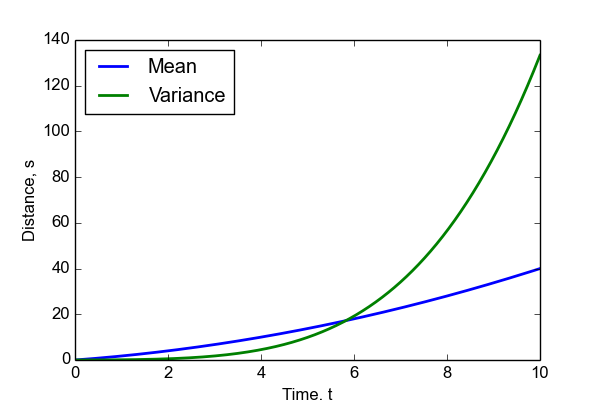
\includegraphics[width=0.85\textwidth]{solution5.png}
 \end{figure}
\end{frame}



 \begin{chaospy}{Traveling with constant acceleration, point collocation with random samples and least squares minimization.}
 \scriptsize
 \begin{lstlisting}[language=Python]
def s(t, v0, a):
    return v0*t + 0.5*a*t**2

v0 = cp.Uniform(1,2)
a = cp.Beta(2,2)
dist = cp.J(v0,a)

t = np.linspace(0,10,1000)
M = 5

P = cp.orth_ttr(M, dist)
nodes = dist.sample(2*len(P))
solves = [s(t, *n) for n in nodes.T]
U_hat = cp.fit_regression(P, nodes, solves,rule="LS")

E = cp.E(U_hat, dist)
Var = cp.Var(U_hat, dist)
\end{lstlisting}
\end{chaospy}


\begin{frame}
 \frametitle{Traveling with constant acceleration, point collocation with random samples and least squares minimization.}
  \begin{figure}
  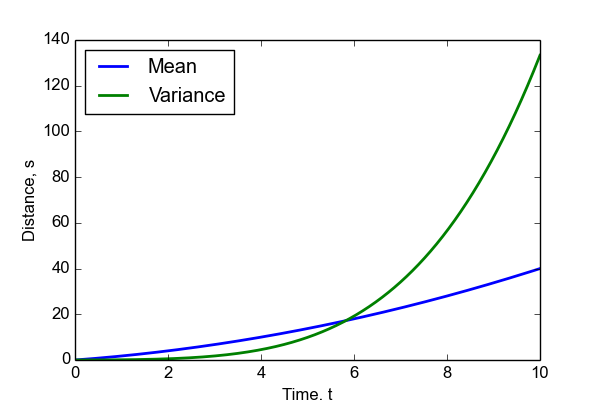
\includegraphics[width=0.85\textwidth]{solution6.png}
 \end{figure}
\end{frame}



 \begin{chaospy}{Traveling with constant acceleration, point collocation with Ha\underline{m}mersley samples and \underline{T}ikhonov regularization.}
 \scriptsize
 \begin{lstlisting}[language=Python]
def s(t, v0, a):
    return v0*t + 0.5*a*t**2

v0 = cp.Uniform(1,2)
a = cp.Beta(2,2)
dist = cp.J(v0,a)

t = np.linspace(0,10,1000)
M = 5

P = cp.orth_ttr(M, dist)
nodes = dist.sample(2*len(P), "M")
solves = [s(t, *n) for n in nodes.T]
U_hat = cp.fit_regression(P, nodes, solves,rule="T")

E = cp.E(U_hat, dist)
Var = cp.Var(U_hat, dist)
\end{lstlisting}
\end{chaospy}


\begin{frame}
 \frametitle{Traveling with constant acceleration, point collocation with Ha\underline{m}mersley samples and \underline{T}ikhonov regularization.}
  \begin{figure}
  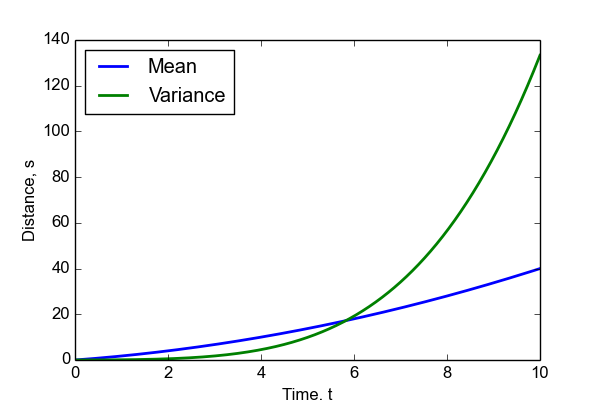
\includegraphics[width=0.85\textwidth]{solution7.png}
 \end{figure}
\end{frame}



\end{document}
